\section{A same-link induced quantum-gravity chain}
\label{sec:same-link-induced-gravity}

The unified-continuum theorem of
Sec.~\ref{sec:unified-operational-continuum} solves a compatibility problem:
one register family can supply order, volume, and an Einstein--matter
response on the same limiting geometry.  It does not solve the origin of the
Einstein--Hilbert coefficient, because the action phase is part of that
model's microscopic update.  This section closes that narrower missing
interface in a different explicit regulator.  No curvature action is placed
in the update.  Scalar matter propagating on the same relational links that
carry order and volume induces a positive two-derivative transverse-
traceless (TT) kernel, and that kernel has a controlled large-species quantum
infrared limit \cite{XuSameLinkInduced2026}.

The result is model-specific.  Four dimensions, a colored graph language, a
low-entropy constructor/clock state, a fair pair scheduler, one physical
volume unit per record, the scalar species, a fixed microscopic spacing, and
the fixed-volume TT sector are declared inputs.  The theorem therefore
removes neither the generic-order assumption A7 nor the universal
capacity-density assumption A9V.  It removes the bare-curvature-action input
only in the displayed TT branch.

\subsection{Anonymous constructor and common record support}

Let
\begin{equation}
 {\cal G}_L=P_L\times T_L^3
 \label{eq:same-link-language}
\end{equation}
be a path of \(L\) clock layers times a periodic cubic spatial graph.
Constant-size gadgets encode its clock and spatial edge colors in a simple
unlabeled graph.  The resulting permutation-invariant language is decidable
in logarithmic workspace: a verifier checks gadget type, consistent layer
increments, periodic three-axis incidence, and the graph-size relation.
Universal stable-network-constructor results then compile an anonymous
finite-state pair protocol whose absorbing output is isomorphic to
\({\cal G}_L\) \cite{MichailSpirakis2016}.  This invokes constructor
universality; it is not a new optimal constructor theorem and does not
dynamically select \(3+1\) dimensions.

For the final relational verification stage, let \(M=n(n-1)/2\) be the
number of unordered pair registers and \(W_r\) the number of wrong edge
bits after \(r\) random pair inspections.  Overwriting the inspected bit by
its relational certificate gives
\begin{equation}
 {\mathbb E}(W_{r+1}\mid W_r)
 =W_r\left(1-\frac1M\right),
 \qquad
 \eta_{\rm con}(s)
 :=\frac{{\mathbb E}W_{sM}}{M}\leq
 \eta_{\rm con}(0)e^{-s}.
 \label{eq:same-link-constructor-error}
\end{equation}
Every stochastic pair transition \(P(c'|c)\) has the exact fresh-cell
isometry
\begin{equation}
 V|c\rangle|0\rangle_E
 =\sum_{c'}\sqrt{P(c'|c)}\,|c'\rangle|c,c'\rangle_E ,
 \label{eq:same-link-stinespring}
\end{equation}
which extends to a unitary and recovers the pair map after the cell is
traced out \cite{Stinespring1955}.  A history-state construction can encode
the finite collision word \cite{Feynman1985,PageWootters1983}; it does not
make the program or clock state dynamical.

The directed clock links generate a partial order after transitive closure.
Each accepted vertex carries one Boolean record cell.  For any record subset
\(A\),
\begin{equation}
 \mu_L(A)=a_*^4\,\# A ,
 \label{eq:same-link-volume}
\end{equation}
which is positive and exactly additive.  For a macroscopic profile
\(F_R(x)=f(x/R)\), \(R=La_*\), midpoint summation yields
\begin{equation}
 \left|
 \frac{a_*^4}{R^4}\sum_{x\in{\cal G}_L}F_R(x)
 -\int_{[0,1]^4}f(u)\,\diff^4u
 \right|
 \leq C_fL^{-2}.
 \label{eq:same-link-volume-rate}
\end{equation}
The same active links define the scalar graph Laplacian.  Its spatial
dispersion is
\begin{equation}
 \widehat{\bm k}^{\,2}
 =\frac4{a_*^2}\sum_{i=1}^{3}
 \sin^2\!\left(\frac{a_*k_i}{2}\right)
 =\bm k^2+O(a_*^2|\bm k|^4).
 \label{eq:same-link-dispersion}
\end{equation}
Thus order, integer volume, and long-wave matter response are not evaluated
on three separately supplied graphs.

\begin{figure}[p]
 \centering
 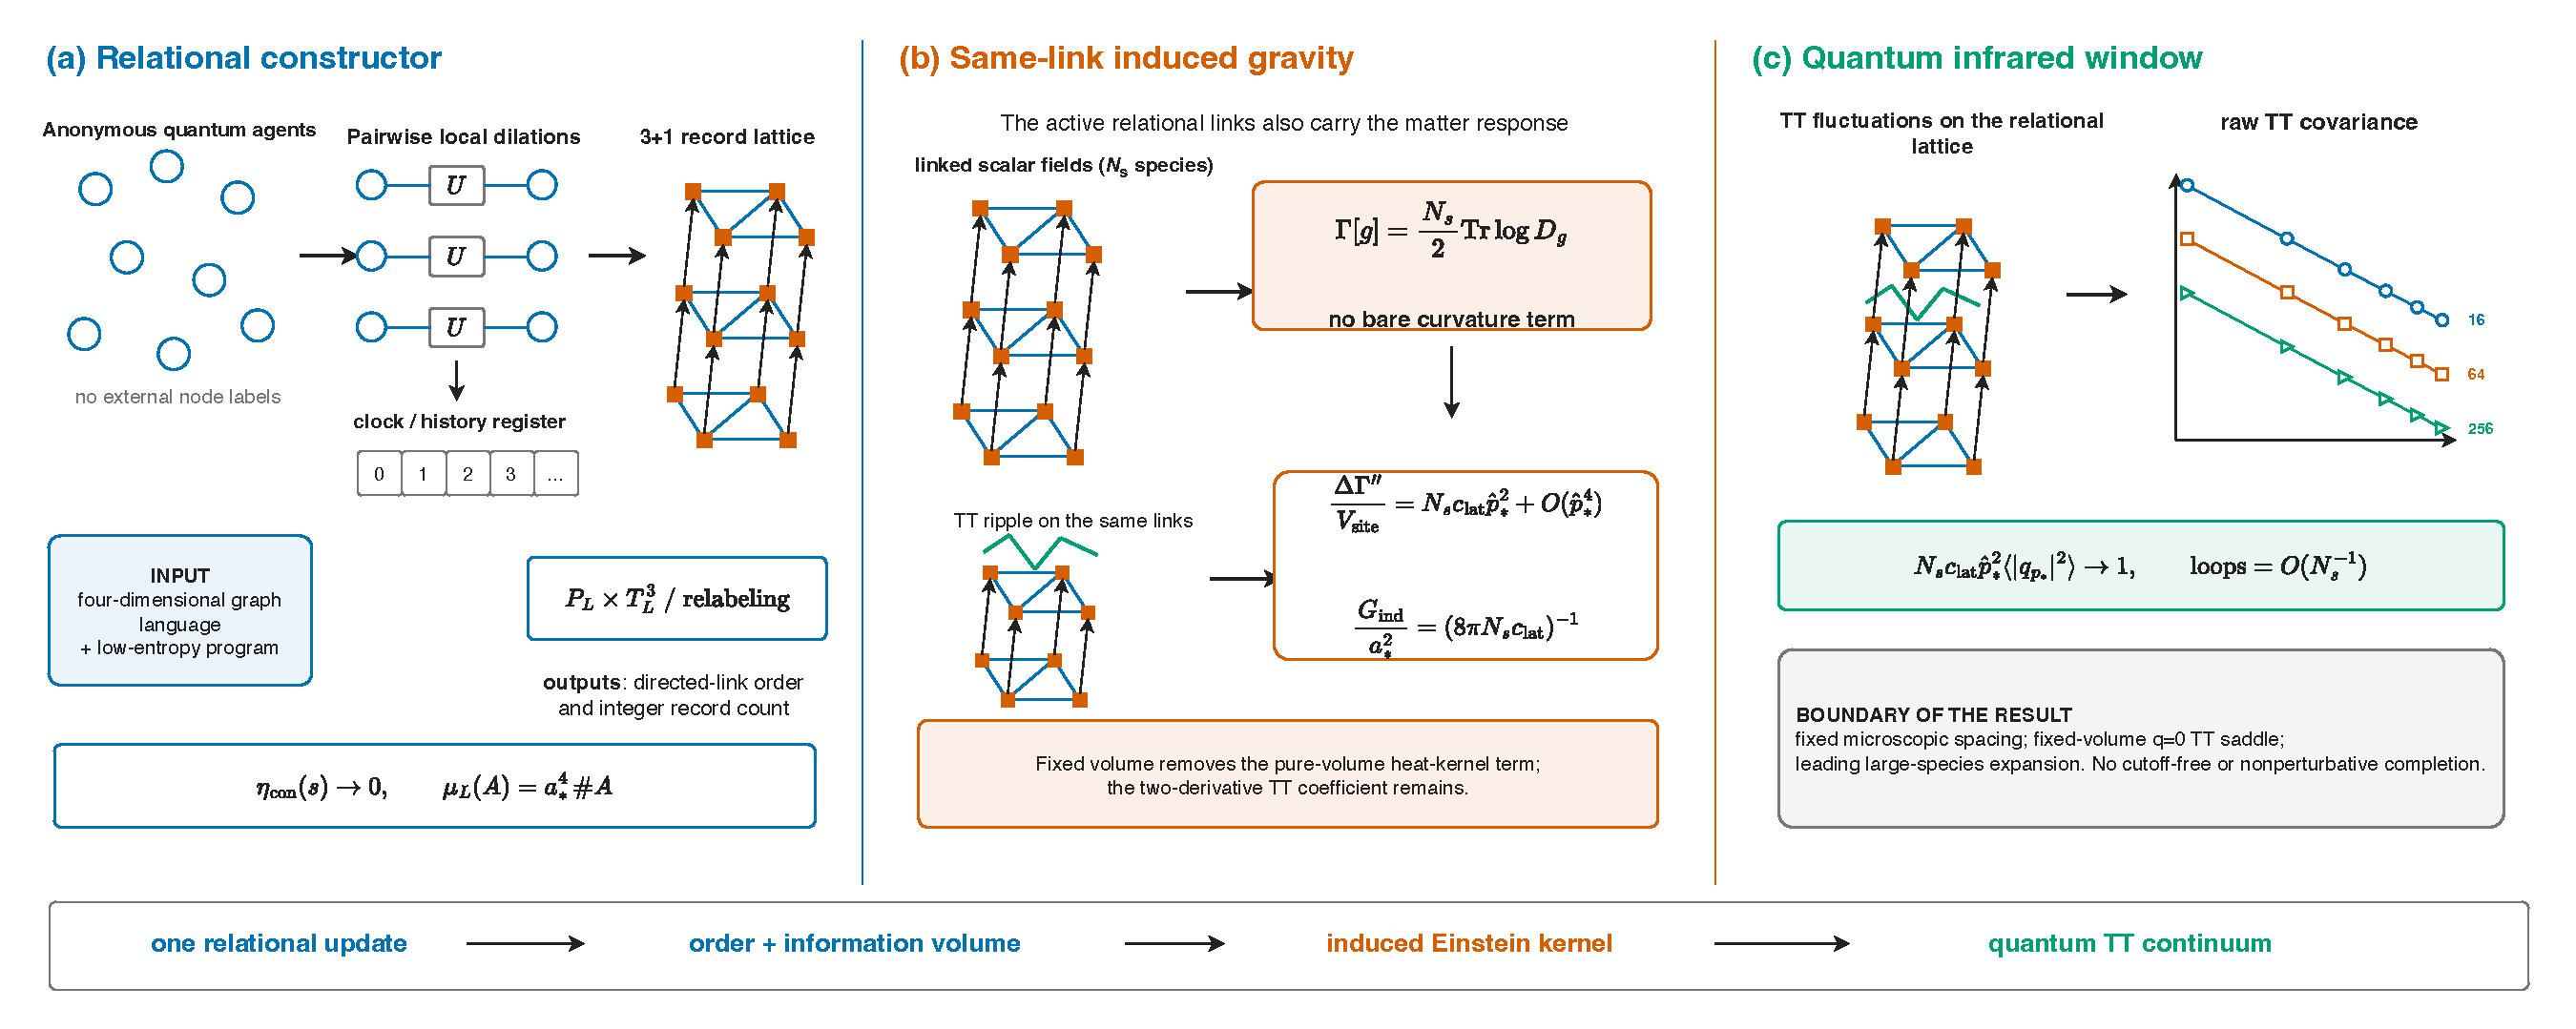
\includegraphics[width=\linewidth]
 {figures/rqcp_qg_same_link_induced_gravity_v1.pdf}
 \caption{\textbf{Model-specific same-link chain.}
 (a) Anonymous local pair interactions compile an unlabeled
 \(P_L\times T_L^3\) record lattice.  The four-dimensional language,
 program/clock state, and scheduler are inputs; order and integer record
 volume are outputs on the absorbed support.
 (b) Linked scalar species propagate on those active edges.  Their
 determinant, with no bare curvature term, induces the positive
 two-derivative TT kernel.
 (c) At fixed microscopic spacing, the rescaled TT covariance approaches a
 Gaussian massless infrared propagator as \(N_s\) increases.  The lower box
 states the boundary that is part of the theorem.  The plotted covariance is
 calculated from the archived regulator, not illustrative data.}
 \label{fig:same-link-mechanism}
\end{figure}

\subsection{Positive Einstein kernel without a bare curvature action}

On the absorbed Euclidean support, take \(N_s\) identical real scalar fields.
Put \(\theta_\alpha=a_*k_\alpha\), \(\mathfrak m=ma_*\), and define the
dimensionless nearest-neighbor operator
\begin{equation}
 D_0(\theta)=\mathfrak m^2+\sum_{\alpha=1}^4\ell_\alpha(\theta),
 \qquad
 \ell_\alpha(\theta)=4\sin^2\frac{\theta_\alpha}{2}.
 \label{eq:same-link-D0}
\end{equation}
The physical operator is \(a_*^{-2}D_0\); its overall power of \(a_*\)
adds only a \(q\)-independent constant to the determinant.
The same link weights carry one plus-polarized, unimodular TT register,
\begin{equation}
 g_{11}=e^{2q\cos(p_*n_4)},\qquad
 g_{22}=e^{-2q\cos(p_*n_4)},\qquad
 g_{33}=g_{44}=1 .
 \label{eq:same-link-TT}
\end{equation}
Here \(p_*=a_*p\) and \(n_4=x_4/a_*\).
Because \(\det g=1\), this perturbation leaves
Eq.~\eqref{eq:same-link-volume} fixed.  Its weighted scalar operator is
\begin{equation}
 D(q)=e^{-2q\cos(p_*n_4)}\ell_1
     +e^{2q\cos(p_*n_4)}\ell_2+\ell_3+\ell_4+\mathfrak m^2 ,
\end{equation}
and the only TT action is the matter determinant
\begin{equation}
 \Gamma[q]=\frac{N_s}{2}\Tr\log D(q).
 \label{eq:same-link-determinant}
\end{equation}

Write \(D=D_0(\theta)\), \(A=\ell_2-\ell_1\), and
\(S=\ell_1+\ell_2\).  For a nonzero cosine mode, direct
differentiation gives, per species and lattice site,
\begin{equation}
 \frac{\Gamma''(p_*)}{N_sV_{\rm site}}
 =\frac12\int_{[-\pi,\pi]^4}\frac{\diff^4\theta}{(2\pi)^4}
 \left[
 \frac{2S}{D}
 -\frac{A^2}{D}
 \left(\frac1{D_{\theta+p_*e_4}}+\frac1{D_{\theta-p_*e_4}}\right)
 \right].
 \label{eq:same-link-exact-kernel}
\end{equation}
The \(p_*=0\) subtraction is taken with the limiting normalization of the
nonzero cosine.  Expanding the shifted resolvents and integrating by parts
in \(\theta_4\) yields
\begin{align}
 \frac{\Gamma''(p_*)-\Gamma''(0)}{N_sV_{\rm site}}
 &=c_{\rm lat}(\mathfrak m)\widehat p_*^{\,2}
   +O(\widehat p_*^{\,4}),\nonumber\\
 c_{\rm lat}(\mathfrak m)
 &=2\int_{[-\pi,\pi]^4}\frac{\diff^4\theta}{(2\pi)^4}
 \frac{(\ell_2-\ell_1)^2\sin^2\theta_4}
 {\left[\mathfrak m^2+\sum_\alpha\ell_\alpha(\theta)\right]^4}>0 .
 \label{eq:same-link-positive-c}
\end{align}
Here \(\widehat p_*^{\,2}=4\sin^2(p_*/2)\) is dimensionless.
Strict positivity follows because the integrand is nonnegative and is
positive on a set of nonzero measure whenever matter hops in both transverse
directions.  It is not inferred from a fit.  Deleting intersite hopping makes
\(\ell_2-\ell_1=0\) and gives the exact zero control.

For the normalization \eqref{eq:same-link-TT}, the Euclidean convention
\begin{equation}
 S_E=-\frac{M_{\rm P}^2}{2}\int\sqrt g\,R
\end{equation}
has quadratic TT response
\(\tfrac12M_{\rm P}^2a_*^2V_{\rm site}
\widehat p_*^{\,2}|q_{p_*}|^2\).
Consequently
\begin{equation}
 M_{\rm P,ind}^2=\frac{N_sc_{\rm lat}}{a_*^2},
 \qquad
 G_{\rm ind}=\frac{a_*^2}{8\pi N_sc_{\rm lat}} .
 \label{eq:same-link-newton}
\end{equation}
This is a determined coefficient of the specified cutoff theory, not a
universal low-energy number.  The heat-kernel interpretation is the usual
Sakharov mechanism: the linked matter determinant produces the curvature
term \cite{Sakharov1968,Adler1982,Visser2002,Vassilevich2003}.  The novelty
claimed here is the exact positive lattice coefficient and its composition
with the relational record support, not induced gravity by itself.
The pure-volume heat-kernel coefficient cancels from the fixed-volume
difference; curvature-squared and nonlocal \(O(\widehat p_*^4)\) terms remain.
This cancellation is not a vacuum-energy sequestering theorem.

\begin{theorem}[Same-link induced Einstein kernel]
\label{thm:same-link-induced-kernel}
For the scalar operator \eqref{eq:same-link-D0} on an absorbed relational
lattice, the fixed-volume TT determinant has no \(p_*^0\) response and has the
strictly positive leading coefficient
\eqref{eq:same-link-positive-c}.  Hence the induced Newton coefficient
\eqref{eq:same-link-newton} is finite and positive at fixed \(a_*\).
Heavy linked matter decouples as \(ma_*\to\infty\), whereas an ultralocal
matter control gives \(c_{\rm lat}=0\).
\end{theorem}

\subsection{Quantum infrared limit of the induced field}

Integrate the TT link register on the perturbative basin of the stable
\(q=0\) saddle with a translation-invariant local reference measure and the
determinant action \eqref{eq:same-link-determinant}.  Around that saddle,
\begin{equation}
 \Gamma[q]
 =N_s\sum_{n\geq2}\frac1{n!}\Gamma_n[q^n],
 \qquad
 \Gamma_2(p_*)=c_{\rm lat}\widehat p_*^{\,2}
 \left[1+O(\widehat p_*^{\,2})\right].
 \label{eq:same-link-vertices}
\end{equation}
With \(\varphi_{p_*}=\sqrt{N_sc_{\rm lat}}\,q_{p_*}\),
\begin{equation}
 N_sc_{\rm lat}\widehat p_*^{\,2}
 \langle|q_{p_*}|^2\rangle
 =1+O(\widehat p_*^{\,2})+O(N_s^{-1}).
 \label{eq:same-link-covariance}
\end{equation}
The \(n\)-point vertex of \(\varphi\) scales as
\(N_s^{1-n/2}\), and every additional metric loop costs \(N_s^{-1}\).
Thus connected non-Gaussian cumulants vanish for \(n>2\) on the declared
fixed infrared band.  Reflection positivity of the leading
nearest-neighbor Gaussian kernel gives its standard
Osterwalder--Schrader continuation \cite{OsterwalderSchrader1973}; the
statement is only for this TT field, not for a gauge-complete graviton.

Let \({\cal P}_{\Lambda,L}\) be a finite set of nonzero modes with
\(\max_{p\in{\cal P}_{\Lambda,L}}a_*|p|\to0\), and define
\begin{align}
 \epsilon_{\rm det}(L,\Lambda)
 &=\sup_{p\in{\cal P}_{\Lambda,L}}
 \left|
 \frac{\Gamma_2(p_*)}
 {c_{\rm lat}\widehat p_*^{\,2}}-1
 \right|,\nonumber\\
 {\mathfrak Q}_{L,s,N_s}
 &=\eta_{\rm con}(s)+C_{\rm vol}L^{-2}
 +C_{\rm disp}L^{-2}
 +\epsilon_{\rm det}(L,\Lambda)
 +\epsilon_{\rm BZ}+N_s^{-1}.
 \label{eq:same-link-joint-certificate}
\end{align}
Here \(\epsilon_{\rm BZ}\) is the deterministic Brillouin-zone quadrature
error.  Every summand is either a finite observable or a remainder with a
declared norm.

\begin{theorem}[Composed relational quantum TT limit]
\label{thm:same-link-quantum-limit}
Run the constructor so that \(\eta_{\rm con}\to0\), take \(L\to\infty\) at
fixed \(a_*\) with \(a_*|p|\to0\) on the probed band, refine the
Brillouin-zone quadrature, and take \(N_s\to\infty\).  Then the normalized
integer record measure and graph response converge on their declared
macroscopic tests; the scalar determinant on those same links converges in
the TT sector to the Einstein two-derivative kernel with coefficient
\eqref{eq:same-link-newton}; and every saddle-selected finite-dimensional
Schwinger function of \(\varphi\) on the probed band converges to that of a
massless Gaussian field.  Connected \(n>2\) cumulants are
\(O(N_s^{1-n/2})\), and the composed error is
\(O({\mathfrak Q}_{L,s,N_s})\).
\end{theorem}

The order of limits is part of the theorem.  It is an infrared scale-
separation limit at fixed microscopic spacing, followed by the controlled
large-\(N_s\) expansion.  It is not the removal of a UV cutoff at fixed
physical \(G\).

\subsection{Independent finite certificate and controls}

The canonical calculation checks every interface separately before applying
the composition theorem.  Eight independent relabelings give a maximum
graph-spectrum residual \(6.04\times10^{-14}\); the wrong-link fraction after
ten sweeps is \(2.05\times10^{-5}\), compared with the exact expectation
\(2.28\times10^{-5}\).  The explicit Stinespring isometry and induced channel
have zero residual at numerical precision.  The normalized volume and
dispersion errors scale as \(L^{-1.99997}\) and \(L^{-1.98997}\).

Independent positive-integrand quadrature gives
\begin{equation}
 c_{\rm lat}(ma_*=10^{-3})=0.0029784498 .
 \label{eq:same-link-numerical-c}
\end{equation}
The finite-\(p\) joint extrapolation gives \(0.0029784389\), while the first
periodic momentum gives \(0.00297180\); these are cross-checks rather than
definitions of the coefficient.  At \(N_s=64\) and \(a_*=1\),
\(G_{\rm ind}/a_*^2=0.2087324\).  Raising the lattice mass to \(ma_*=8\) suppresses
\(c_{\rm lat}\) to \(5.07\times10^{-5}\) of its light-mass value.  In the
declared \(L=48\) band, the largest finite-momentum covariance-collapse
error for \(N_s=64\) is \(6.80\%\); the expansion parameter for metric loops
is \(1/64\).

\begin{figure}[p]
 \centering
 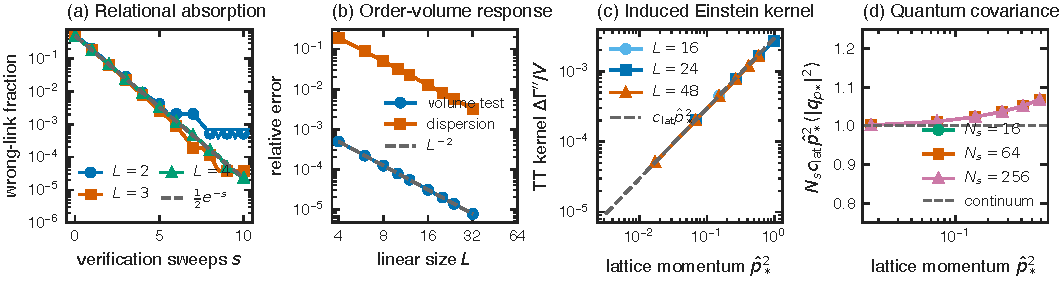
\includegraphics[width=\linewidth]
 {figures/rqcp_qg_same_link_joint_certificate_v1.pdf}
 \caption{\textbf{Independent certificate for the composed limit.}
 (a) Random-pair verification after vertex relabeling.
 (b) Macroscopic record-volume quadrature and linked scalar dispersion.
 (c) The subtracted determinant and its positive
 \(c_{\rm lat}\widehat p_*^2\) limit.
 (d) Collapse of the rescaled TT covariance for three species numbers.
 Open downward markers in panel (a) denote zero observed errors plotted at
 half the aggregate detection floor.}
 \label{fig:same-link-joint-certificate}
\end{figure}

The coefficient has two sharp controls.  It decreases with the linked
matter mass, and it vanishes exactly when intersite hopping is removed.
These distinguish a genuine link-metric response from a fitted positive
constant.  The numerical tables and the scripts used to reproduce the
calculation are provided with the supporting material.

\subsection{What this closes, and what remains}

The model closes the following chain:
\begin{equation}
 \boxed{\begin{gathered}
 \text{anonymous local pair process}\\
 \Downarrow\\
 \text{one unlabeled record support carrying order, integer volume,
 and matter response}\\
 \Downarrow\\
 \text{strictly positive induced TT Einstein kernel}\\
 \Downarrow\\
 \text{controlled saddle-selected fixed-band large-\(N_s\) quantum TT field}.
 \end{gathered}}
 \label{eq:same-link-closed-chain}
\end{equation}
The action and quantum covariance are therefore no longer validated on
microscopic supports unrelated to the order--volume records.

Five boundaries prevent this theorem from being promoted to a general
quantum-gravity result.
\begin{enumerate}
\item The constructor compiles a four-dimensional graph language; it does
not select dimension or topology as a thermodynamic phase.
\item The program/clock state, fair scheduler, orientation color, and record
volume unit \(a_*^4\) remain microscopic inputs.
\item Matter is integrated out after the record support forms.  Its
backreaction on graph formation and a fully autonomous arrow of time are
absent.
\item Only the perturbative basin of the stable \(q=0\), fixed-volume TT
polarization is quantized.  Competing metric saddles, lapse, shift,
scalar/vector constraints, ghosts, nonlinear diffeomorphism symmetry,
caustics, and realistic gauge/fermion matter are not included.
\item The continuum statement keeps \(a_*\) fixed.  Higher-curvature
operators remain, and no regulator-independent trajectory for \(G\) or
cutoff-free quantum measure is established.
\end{enumerate}

Accordingly, A11I is marked \StatusModel, whereas A7, A9V, A11, and A19
remain open.  The next mathematical target is a phase-selection theorem that
replaces the compiled language and clock, followed by a constraint-complete
induced metric measure whose renormalization makes a regulator-independent
prediction.  The present chain is the model-level bridge on which that
stronger theorem must improve.
